\documentclass[11pt]{article}
% packages
% Fran Burstall's Bath thesis package
\usepackage{baththesis}
\usepackage{amssymb} %for Blackboard bold etc \usepackage{graphicx} %for including eps graphics % front matter
\usepackage[pdftex]{graphicx} % To include pictures
\usepackage{caption}
\usepackage{subcaption} % To use subfigures with subcaptions
\usepackage{url}
\usepackage{amsmath} % Equations
\usepackage{txfonts}
\setlength{\parskip}{0.9em} %Paragraph spacing
\usepackage{pgfgantt}
\usepackage{cite}
\usepackage{csquotes}
\renewcommand*{\mkcitation}[1]{ #1}

\newcommand{\phim}{\mathbf{\phi}}
\newcommand{\X}{\mathbf{X}}
\newcommand{\x}{\mathbf{x}}
\newcommand{\Y}{\mathbf{Y}}
\newcommand{\y}{\mathbf{y}}
\newcommand{\w}{\mathbf{w}}
\newcommand{\Z}{\mathbf{Z}}
\newcommand{\z}{\mathbf{z}}
\newcommand{\h}{\mathbf{h}}
\newcommand{\dd}{\: \mathrm{d}}

%\usepackage[hidelinks]{hyperref} % Adds references links without color
\usepackage{hyperref} % Adds references links with color
\usepackage{xcolor}
\hypersetup{
    colorlinks,
    linkcolor={red!50!black},
    citecolor={blue!50!black},
    urlcolor={blue!80!black}
}

\title{Visual Effects} \author{Ieva Kazlauskaite, Garoe Dorta-Perez, Richard Shaw}
%\degree{Doctor of Philosophy}
\unit{ unit }
\department{Department of Computer Sciences} \degreemonthyear{May 2015}
\norestrictions

\begin{document}
\maketitle

\section{Introduction}
\label{ch:intro}
\begin{center}
\textquote[~\cite{Attenborough:1998}]{\textit{Birds are the most accomplished aeronauts the world has ever seen. They fly high and low, at great speed, and very slowly. And always with extraordinary precision and control}.}
\end{center}


\section{Previous Work}
\label{sec:previous}

\subsection{Data Capture}

%-----------------------------------------------------------------------
\subsection{Sparse Reconstruction}


%-----------------------------------------------------------------------
\subsection{Blendshape Optimisation}
In this section we introduce the techniques used to warping the meshes and the optimisation methods.

\subsubsection{Thin Plate Splines}
Thin plate theory deals with problems that commonly arise in areas of natural sciences and engineering when trying to model the behaviour of a thin sheet of some material. The possible processes include but are not limited to stretching, bending, crumpling, buckling, shrinking, straining and tearing. The corresponding mathematical model is based on ideas from differential geometry, and the set of equations describing the aforementioned phenomena are often notoriously difficult to solve. Therefore, in Computer Graphics, as well as other fields, a number of simplifying assumptions are made when constructing a thin plate model. 

A thin plate is considered to be a two dimensional object, i.e. it is assumed that the thickness is infinitesimal. The geometry of the object is often simplified to reduce the computational cost. Thin plate splines (TPS) are a two-dimensional counterpart of the cubic spline. TPS are a deformation method based on the assumption that a thin surface deforms in a way that minimises the surface bending energy. The bending energy is proportional to the change in the second fundamental form. Specifically, given two corresponding sets of point $\{\y_i\}_i^N$ and $\{\x_i\}_i^N$ there exists a height field mapping between the two, $f: \mathbb{R}^2 \to \mathbb{R}$. The bending energy corresponding to this mapping is proportional to the second order derivatives of the mapping:
\begin{equation}
\begin{aligned}
	E_{bend}(f) = \lambda \iint \left( \left( \dfrac{\delta^2f}{\delta x^2} \right)^2 +  2 \left( \dfrac{\delta^2f}{\delta x y} \right)^2 +  \left( \dfrac{\delta^2f}{\delta y^2} \right)^2 \right) \dd x \dd y,
\end{aligned}
\end{equation} where $\lambda$ is smoothing parameter, which balances the quality of fit and the amount of bending, i.e. the wiggliness of the function. TPS finds the transformation that fits the data while minimising the bending energy. Note that TPS may also be defined in terms of the radial basis functions that are used for smooth scattered data fitting. The RBF solution for thin plate splines is:
\begin{equation}
\begin{aligned}
	f(x,y) = \sum_{i=1}^N \alpha_i \: \phi(\|(x,y) - (x_i,y_i)\|), \: \text{ where} \: \phi(r) = r^2 \log(r).
\end{aligned}
\end{equation} To ensure that the function $f$ has square-integrable second derivatives, the following conditions are imposed:
\begin{equation}
	\sum_{i=1}^N \alpha_i = \sum_{i=1}^N \alpha_i x_i = \sum_{i=1}^N \alpha_i y_i = 0.
\end{equation}

\subsubsection{Non-Rigid ICP}


\subsubsection{Numerical Solvers}



%-----------------------------------------------------------------------
\subsection{Skin Rendering}

Rendering realistic skin is a challenging task.
As social beings we interact with interact with other individuals on a daily basis, which has made human perception quite sensitive to skin appearance, even more so with human faces.
Skin is composed of several layers with different properties, to accurately simulate skin the light transport between this layers has to be simulated.
The full effect of light scattering between two points on the surface can be modelled using a Bidirectional Surface-Scattering Distribution Function (BSSRDF).

Weyrich et al~\cite{Weyrich2006} proposed a two-layer model for skin rendering, the outer layer simulates the air-oil interface and the inner layer models the subsurface scattering in the skin.
The authors considered the scattering to be homogeneous, with this assumption they measured the skin BRDF of several subjects in a light dome, while the scattering was sampled at three points in the face with a custom made sensor.
The BRDF data was fitted to a Blinn-Phong and a Torrance-Sparrow isotropic models, and the scattering was fitted with a single transport coefficient.
Donner et al~\cite{Donner2008} also proposed a two-layer model, however the authors allow for the layers to be heterogeneous.
With this addition they are able to introduce the effects of haemoglobin, veins and tattoos.
Emotional induced haemoglobin variations have also been explored ~\cite{Jimenez2010}.
The authors measured the haemoglobin distributions of several subjects in different poses, then a linear combination of the captured data would determine the final haemoglobin distribution for a new sequence.
Recently, Iglesias et al~\cite{Iglesias2015} introduced a five-layer model to handle skin ageing.
Haemoglobin, collagen and fat changes with age are modelled using the different layers.

Normal maps are use to alter the normals of the scene objects during rendering.
This technique is used to add geometric detail to an object at rendering time without actually changing the geometry.
%The error introduced with this approach is shown in Figure \ref{fig:normal_map}, a ray $r_1$ hist the geometry at point $p$ and the normal $n_p$ is used for shading, while if we had the based geometry the hitting point would be $p'$ and the normal $n'$.
Normal maps for skin rendering are usually captured using expensive light domes with a number of synchronized cameras ~\cite{Graham2013, Weyrich2006}. 

Another technique to increase the quality of a face render is to scale the resolution of the textures being used.
Ashikhmin et al~\cite{Ashikhmin2001} presented a method to generate new textures using a goal image by greedily extending existing patches whenever possible.
Hertzmann et al~\cite{Hertzmann2001} extended Ashikhmin et al~\cite{Ashikhmin2001} method by adding a second example image and using more complex distance metric to choose the next synthesized pixel.
Graham et al~\cite{Graham2013} applied Hertzmann et al~\cite{Hertzmann2001} example-based filter to generate bump maps with increased quality for skin rendering.
An alternative approach using a dictionary of samples was presented by Jianchao et al~\cite{Jianchao2010}.
This method is restricted to generating super-resolution images, however, the previous methods support a wide variety of filter effects.
For an in depth analysis of super-resolution techniques, we refer the readers to Tian et al~\cite{Tian2011} survey.

%\begin{figure}[htbp!]
%\centering
%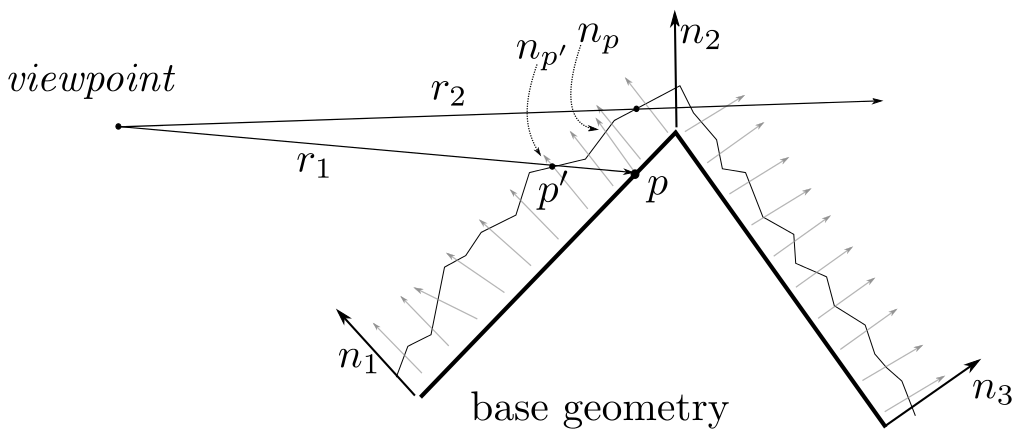
\includegraphics[width=0.7\textwidth]{img/normal_map}
%	\caption{ Using normal maps to simplify a given geometry, image taken from \cite{ganovelli2014}.}
%	\label{fig:normal_map}
%\end{figure}



%-----------------------------------------------------------------------
\section{Methodology}
\label{sec:methods}


\subsection{Data Capture}


\subsection{Sparse Reconstruction}


\subsection{Blendshape Optimisation}


\subsection{Skin Rendering}

\subsection{Skin Rendering}

Our objective in skin rendering is to generate a face that would indistinguishable from a real one.
To be more specific, we have have taken a 3D scan of a subject and our aim is to improve the realism of it.
For this task we will mainly look at the techniques presented by Hertzmann et al~\cite{Hertzmann2001} and Graham et al~\cite{Graham2013}.

Before we begin, lets explain the Image Analogies framework~\cite{Hertzmann2001} in more detail.
Given three images $A$, $A'$ and $B$, where $A$ is an unfiltered example, $A'$ is a filtered example, and $B$ is an input image, the algorithm will generate an output image $B'$ such that $B'$ relates in the same way to $B$ as $A'$ does to $A$, as shown in Figure~\ref{fig:ia_diagram}.
A k-d tree for an Approximate Nearest-Neighbour Search (ANN) is built using a feature vector from a neighbour pixel $p$ in $A$ and $A'$.
The closest match for a neighbourhood in pixel $q$ in $B$ and $B'$ is located in the tree.
Following Ashikhmin et al~\cite{Ashikhmin2001} method, a match that is coherent to what has been already synthesized is computed as well.
These two candidates are weighted and the best one is chosen.
The whole process is carried in a multiresolution pyramid, as shown in Figure~\ref{fig:ia_diagram}, where $l$ indicates the current level, in essence what this means is that the neighbourhoods also include the previous level in the search.

\begin{figure}[htbp!]
\begin{minipage}[b]{.55\textwidth}
\centering
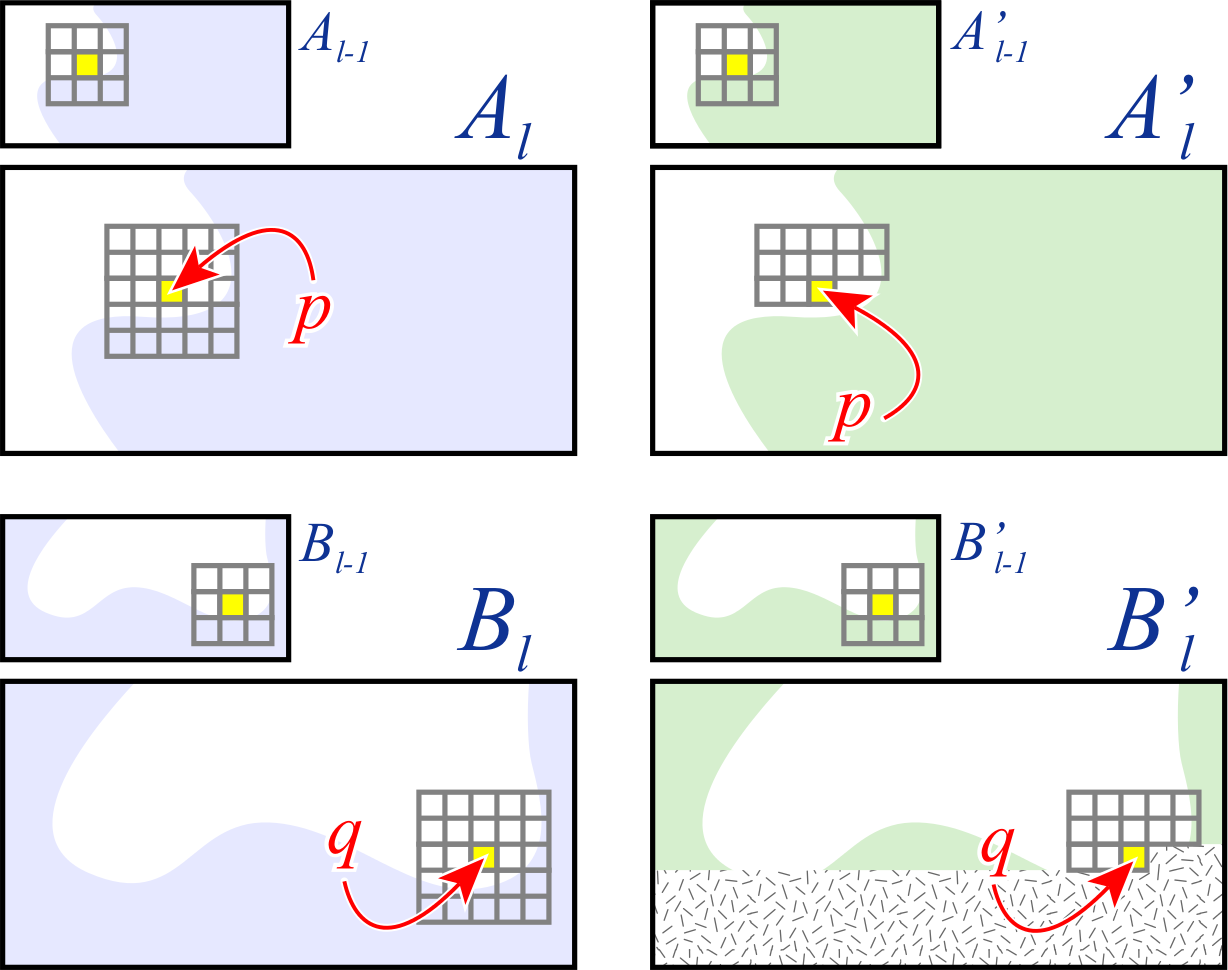
\includegraphics[width=\textwidth]{img/ia_diagram}
	\caption{ Neighbourhood matching for the Image Analogies framework, image taken from~\cite{Ashikhmin2001}.}
	\label{fig:ia_diagram}
\end{minipage}
\hfill
\begin{minipage}[b]{.4\textwidth}
\centering
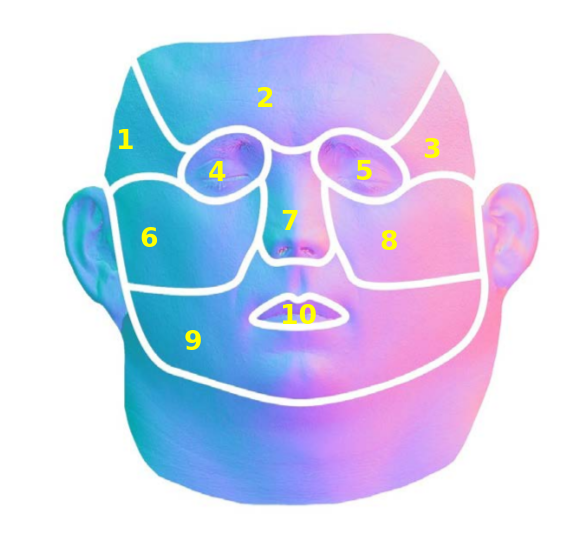
\includegraphics[width=\textwidth]{img/texture_synthesis_parts}
	\caption{ Texture segmentation in common coloured areas, image taken from~\cite{Graham2013}.}
	\label{fig:texture_synthesis_parts}	
\end{minipage}
\end{figure}

As a first approach we tried to reproduce the results in bump mapping quality increase by Graham et al~\cite{Graham2013}.
The authors add am extra $alpha \in \left\lbrace 0, \ldots, 1 \right\rbrace$ parameter to control Hertzmann's image synthesis process.
In more detail, a match between $A$ and $\left\lbrace B,B' \right\rbrace$ will be weighted by $1 - \alpha$, while a match between $A'$ and $\left\lbrace B,B' \right\rbrace$ will be weighted by $\alpha$.
The logic behind this addition is to encourage more details of $A'$ to be included in $B'$.
The modifications include building two separated k-d trees for $A$ and $A'$ and then doing the appropriate weighting when choosing the pixel position.
Also in the coherence match two searches will be done and weighted accordingly, and the final pixel will be chosen without further adjustments.
ADD BUMP MAP IMAGE OR NOT IF THERE IS NOT ENOUGH SPACE

Another approach we tried was to use the Image Analogies filter to create increase quality textures.
We found three implementations available \cite{ImAnSingleThreadWeb, ImAnCudaWeb, ImAnHertzmannWeb}.
The second one was done with CUDA, however the author's single threaded code gave better results.
The idea in this approach is to use a low quality texture from a 3D scan and improve using pictures of the texture at a closer range.
To achieve this we took a close up high quality sample $A'$, which was blurred using a Gaussian kernel until it look qualitative similar to the 3D scan texture $B$.
The blurred image is $A$ and then we generated a picture $B'$ of higher quality.
Since faces have differentiated areas, this process was done separately for each of them, the generated patches are then stitched together using linear interpolation.
The texture segmentation is shown in Figure~\ref{fig:texture_synthesis_parts} and results are shown in Figure~\ref{fig:texture_synthesis}.

\begin{figure}[htbp!]
\centering
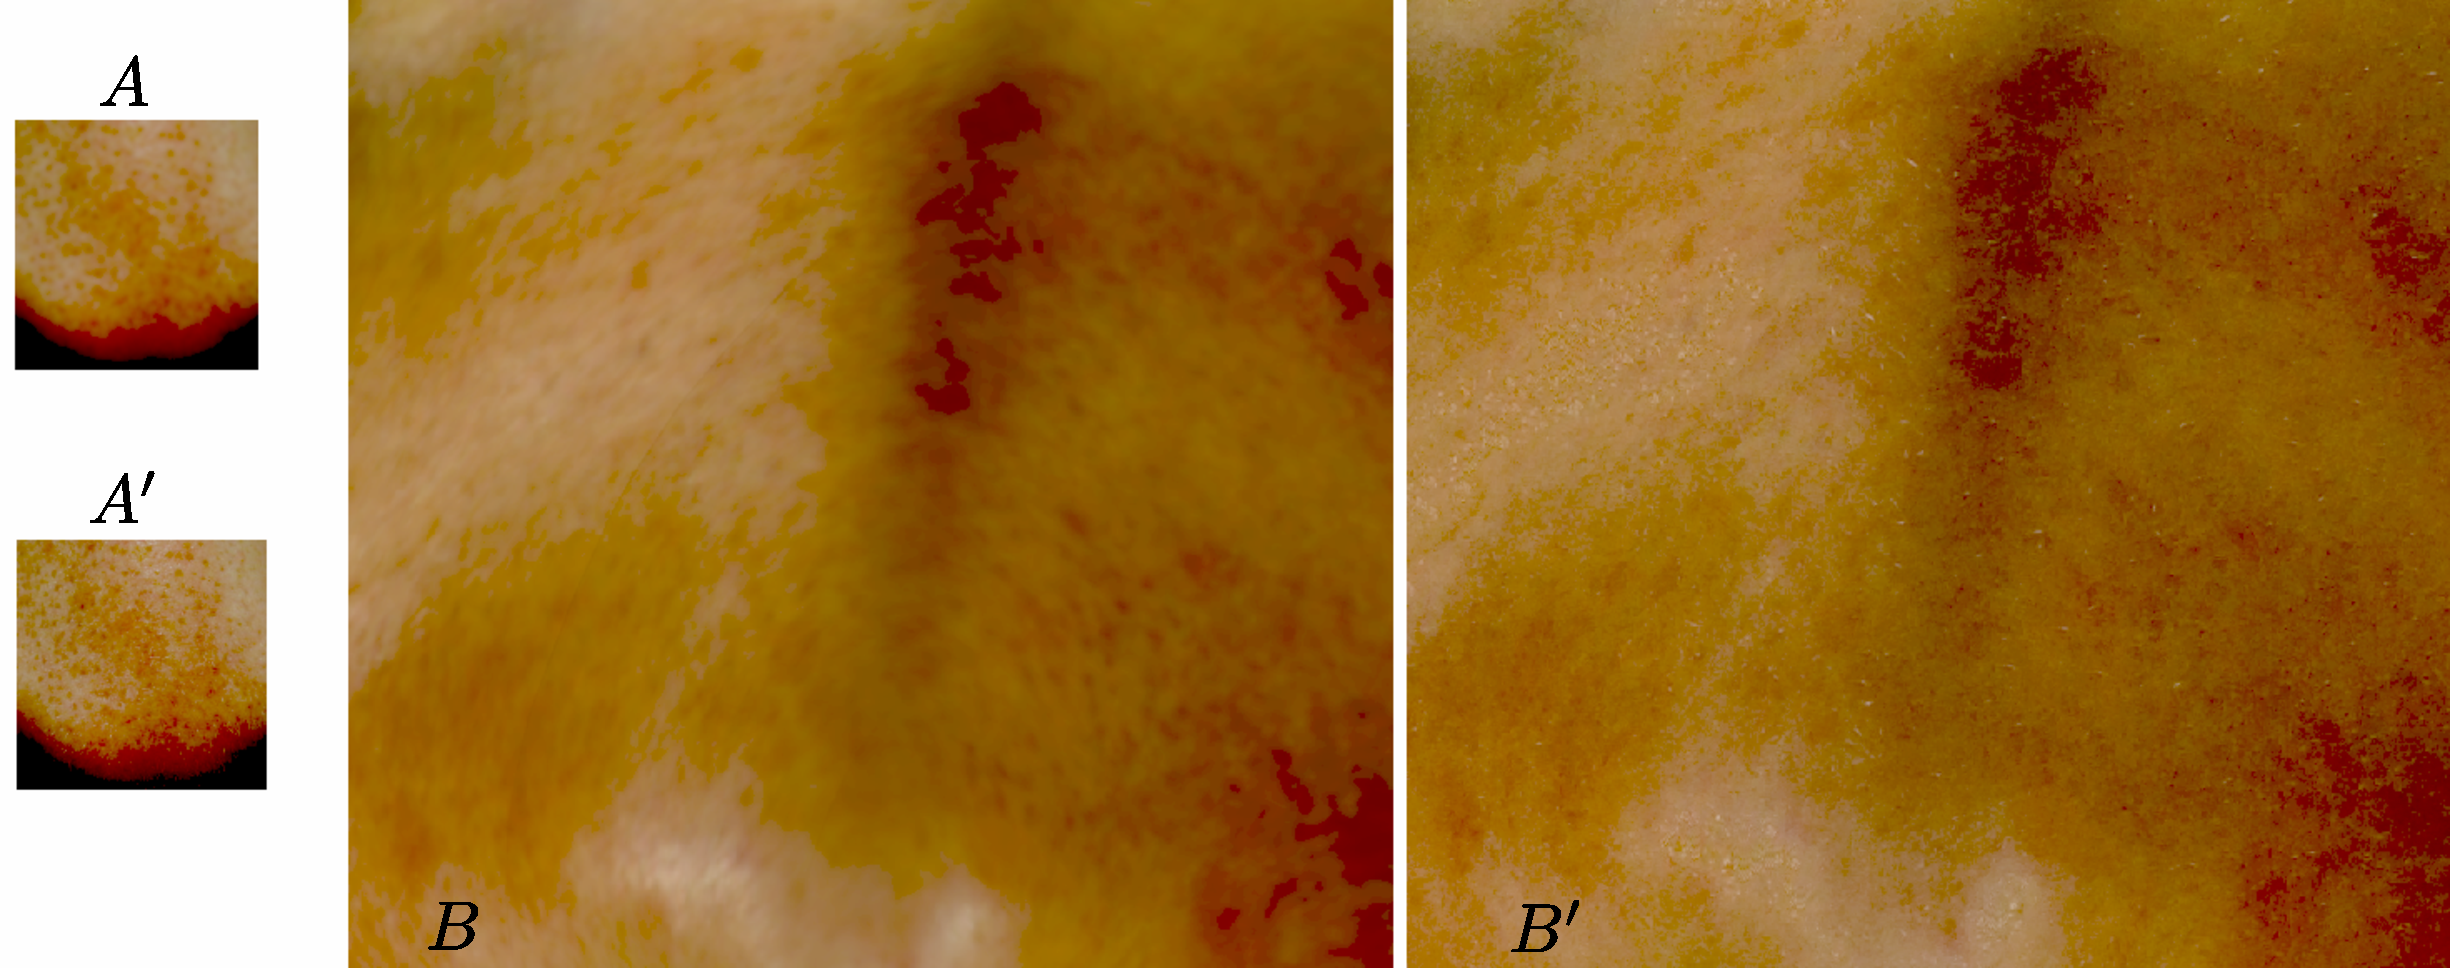
\includegraphics[width=\textwidth]{img/texture_synthesis}
	\caption{ Texture quality increase using image analogies, the texture is false-coloured to highlight the differences.}
	\label{fig:texture_synthesis}
\end{figure}

Another option for increasing the quality of the texture is to use image super-resolution, we used Jianchao et al~\cite{Jianchao2010} work for this purpose.
The idea is that by doubling the resolution of the original texture adding information from a dictionary of high resolution images we will be able to increase the final rendering quality of the face.
Results for this are shown in Figure~\ref{fig:emily_super_resolution}.

\begin{figure}[htbp!]
\centering
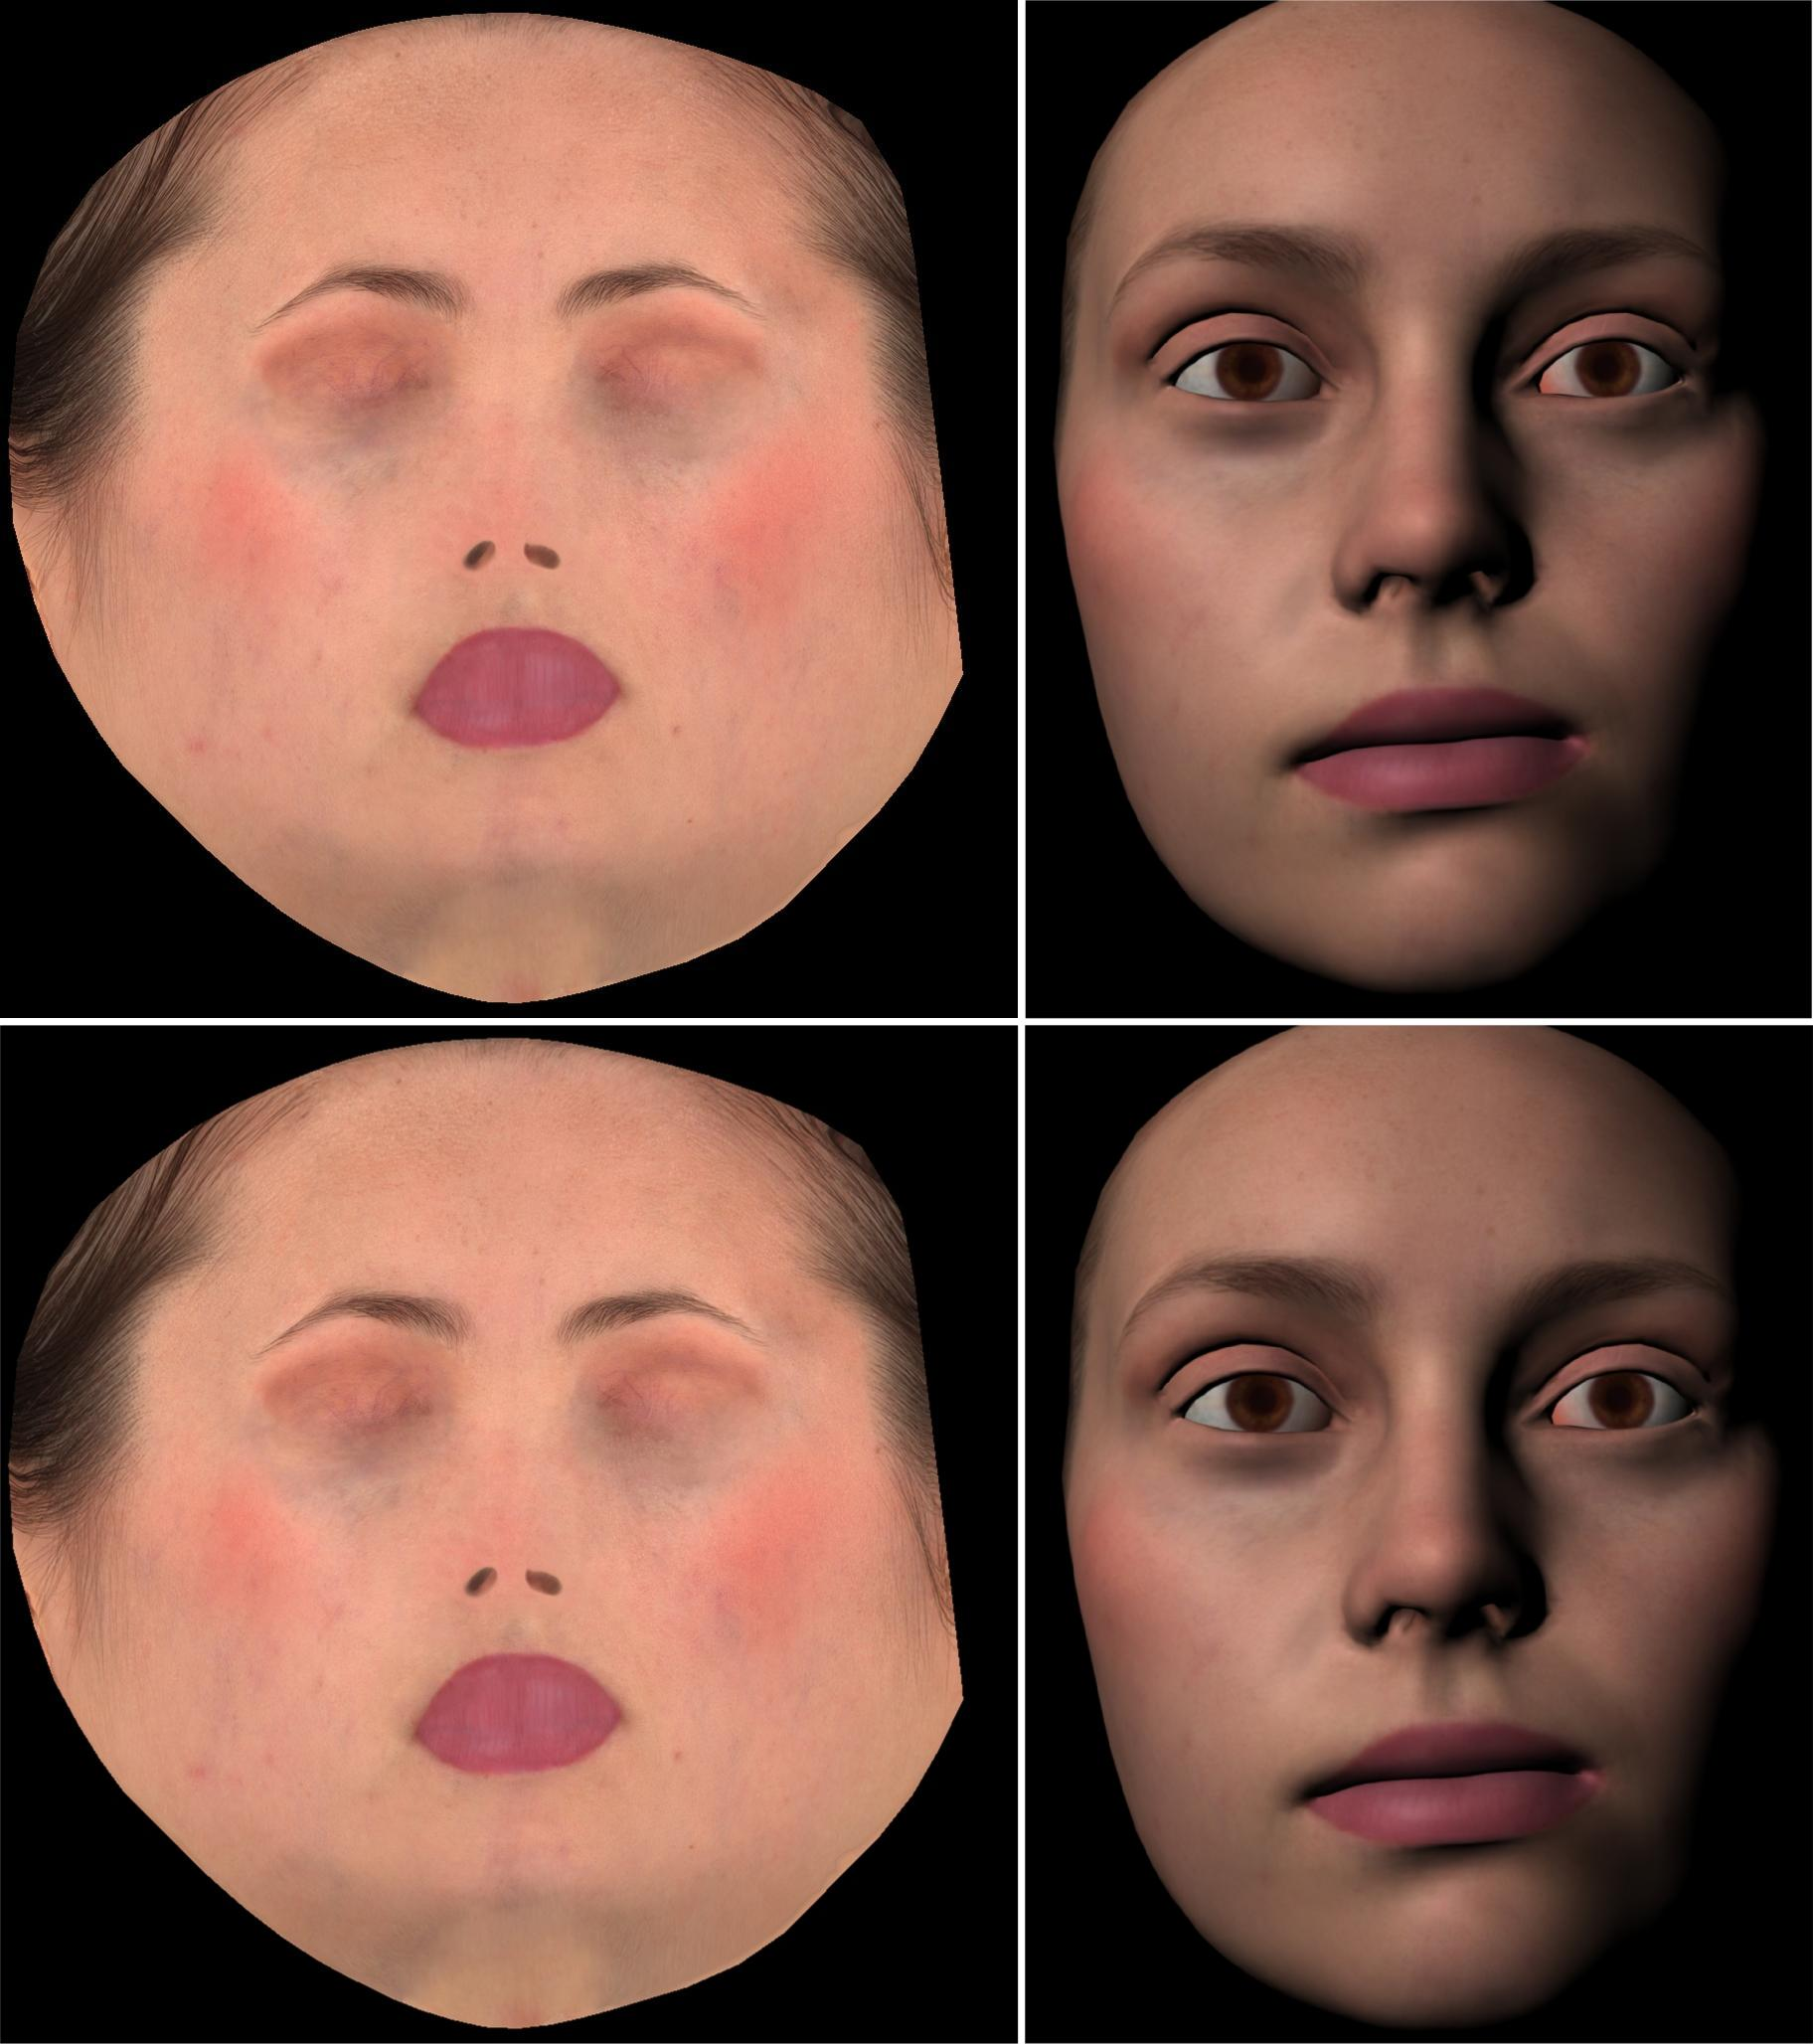
\includegraphics[width=0.6\textwidth]{img/emily_super_resolution}
	\caption{ Super resolution example, top-left original texture, top-right face rendered with original texture, bottom-left super-resolution texture, bottom-right face rendered with super-resolution texture, original data from CITE EMILY DATA.}
	\label{fig:emily_super_resolution}
\end{figure}

Generating normals maps using Image Analogies is another interesting area, as it could provide a way to avoid he costly standard capture methods.
For this we tried to generate a normal map from an albedo images and from bump maps generated from the previous 3D scan texture.
Results for this are shown in Figure~\ref{fig:normal_synthesis}.

\begin{figure}[htbp!]
\centering
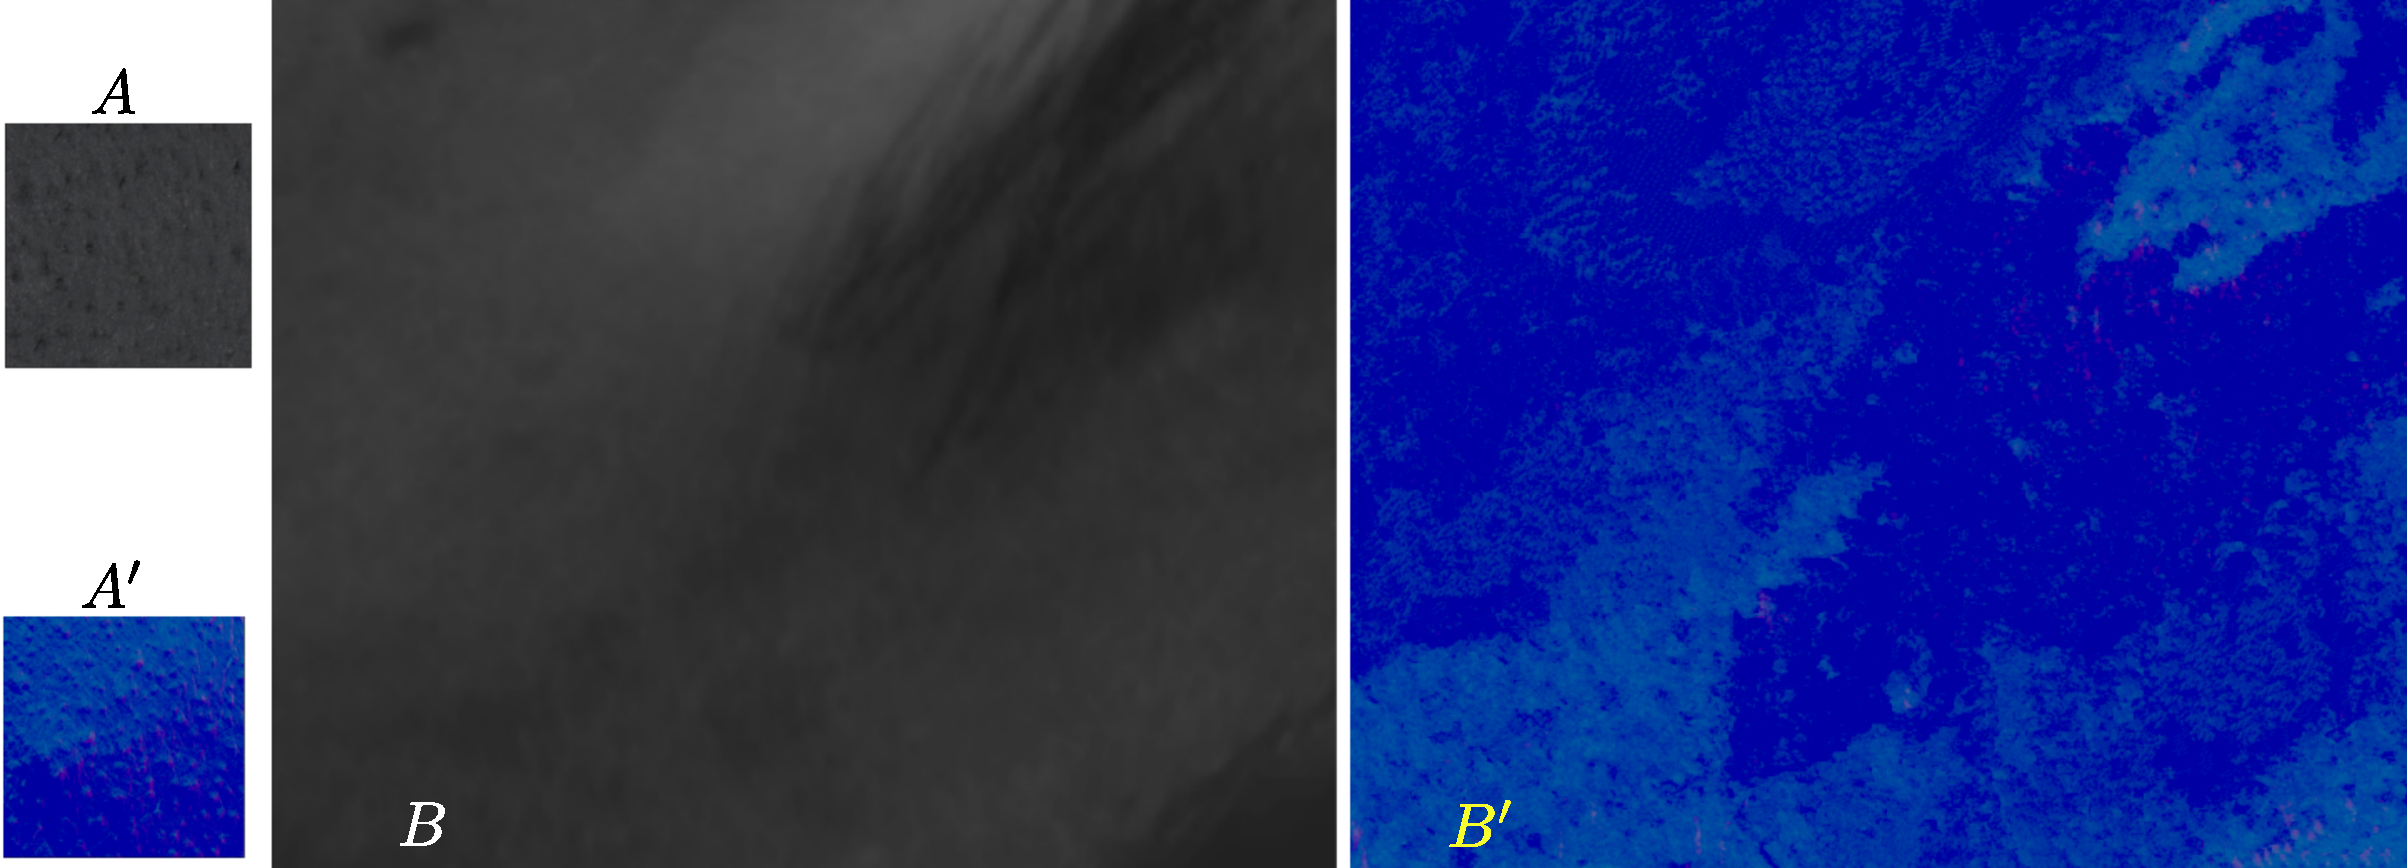
\includegraphics[width=\textwidth]{img/normal_generation}
	\caption{ Normal synthesis from albedo image.}
	\label{fig:normal_synthesis}
\end{figure}

% Things that we tried
% Replicate Graham2013, bump map synthesis
% Bump maps from texture and then bump map increase
% Jianchao work for super resolution
% Adding the alpha to parameter as Graham2013 for the bump maps


%-----------------------------------------------------------------------
\section{Results}


%-----------------------------------------------------------------------
\section{Conclusions}

\bibliographystyle{eg-alpha}
\bibliography{baththesis}

\end{document}